\documentclass[8pt,aspectratio=169]{beamer}
\usepackage[ruled,vlined]{algorithm2e}
\usepackage{amsmath}
\usepackage{amssymb}
\usepackage{amsfonts}
\usepackage{amsthm}
\usepackage{appendixnumberbeamer}
\usepackage[backend=biber, giveninits]{biblatex}
\usepackage{booktabs}
\usepackage{bm}
\usepackage{caption} 
\captionsetup[table]{skip=5pt}
\usepackage[scale=2]{ccicons}
\usepackage{color}
\usepackage{derivative}
\usepackage[inline,shortlabels]{enumitem}
\usepackage{epsfig}
\usepackage{expl3}
\usepackage{graphicx}
\usepackage{hyperref}
\usepackage{makecell}
\usepackage{mathtools}
\usepackage{multicol}
\usepackage{multirow}
\usepackage{placeins}
\usepackage{siunitx}
\usepackage{svg}
\usepackage{times}
\usepackage{xcolor}
\usepackage{xspace}
\usepackage{xparse}

%%%%%%%%% content delimiters
\NewDocumentCommand\secref{m}{Section~{\ref{#1}}}
\NewDocumentCommand\figref{m}{Figure~{\ref{#1}}}
\NewDocumentCommand\tabref{m}{Table~{\ref{#1}}}
\NewDocumentCommand\secsref{m}{Sections~{\ref{#1}}}
\NewDocumentCommand\figsref{m}{Figures~{\ref{#1}}}
\NewDocumentCommand\tabsref{m}{Tables~{\ref{#1}}}
\NewDocumentCommand\algref{m}{Algorithm~{\ref{#1}}}

%%%%%%%%% abbreviations
\makeatletter
\DeclareRobustCommand\onedot{\futurelet\@let@token\@onedot}
\def\@onedot{\ifx\@let@token.\else.\null\fi\xspace}
\def\eg{\emph{e.g}\onedot} \def\Eg{\emph{E.g}\onedot}
\def\ie{\emph{i.e}\onedot} \def\Ie{\emph{I.e}\onedot}
\def\cf{\emph{c.f}\onedot} \def\Cf{\emph{C.f}\onedot}
\def\etc{\emph{etc}\onedot} \def\vs{\emph{vs}\onedot}
\def\wrt{w.r.t\onedot} \def\dof{d.o.f\onedot}
\def\etal{\emph{et al}\onedot}
\makeatother

%%%%%%%%%% colors
\definecolor{mycolor1}{rgb}{0,0,0}%
\definecolor{mycolor2}{rgb}{1,0,1}%
\definecolor{mycolor3}{rgb}{0,1,1}%
\definecolor{mycolor4}{rgb}{0,0,1}%
\definecolor{mycolor5}{rgb}{0,1,0}%
\definecolor{betteryellow}{rgb}{1,0.8824,0.0980}
\definecolor{lavender}{rgb}{0.902,0.7451,1.0}
\definecolor{olive}{rgb}{0.5020,0.5020,0} 
\definecolor{orange}{rgb}{1,0.5,0} 
\definecolor{bettergreen}{rgb}{0,0.6,0.3}

\definecolor{blue}{HTML}{4069B0}
\definecolor{lightorange}{HTML}{FF8F00}
\definecolor{orange}{HTML}{E45611}
\definecolor{darkorange}{HTML}{B85325}
\definecolor{lightgreen}{HTML}{34DC5B}
\definecolor{green}{HTML}{28A745}
\definecolor{lightgray}{HTML}{656972}
\definecolor{gray}{HTML}{53585F}
\definecolor{darkgray}{HTML}{333333}
\definecolor{red}{HTML}{D61901}
\definecolor{magenta}{HTML}{CC00CC}
\definecolor{cyan}{HTML}{00FFFF}

\def\firstpl#1{\textcolor{bettergreen}{\textbf{#1}}}
\def\secondpl#1{\textcolor{lightorange}{\textbf{#1}}}
\def\stateofart#1{\textbf{#1}}
\def\red#1{\textcolor{red}{\textbf{#1}}}

\newcommand{\mycbox}[1]{\tikz{\path[draw=#1,fill=#1] (0,0) rectangle (5pt,5pt);}}
\DeclareMathOperator{\rank}{rank}%
\DeclareMathOperator{\vect}{vec}%
\DeclareMathOperator{\atantwo}{atan2}%
\DeclareMathOperator*{\argmin}{argmin}%
\DeclareMathOperator*{\argmax}{argmax}%

\DeclarePairedDelimiter{\abs}{\lvert}{\rvert}
\DeclarePairedDelimiter{\norm}{\lVert}{\rVert}
\DeclarePairedDelimiter{\innerproduct}{\langle}{\rangle}

\DeclarePairedDelimiter{\parenfences}{(}{)}
\DeclarePairedDelimiter{\brackets}{[}{]}
\DeclarePairedDelimiter{\coord}{(}{)}
\DeclarePairedDelimiterX{\sksym}[1]{[}{]_{\times}}{#1}

% just to make sure it exists
\providecommand\given{}
% can be useful to refer to this outside \Set
\newcommand\SetSymbol[1][]{%
\nonscript\:#1\vert
\allowbreak
\nonscript\:
\mathopen{}}

\DeclarePairedDelimiterX\set[1]\{\}{%
\,\renewcommand\given{\SetSymbol[\delimsize]}
#1\,
}

\NewDocumentCommand\Zz{}{\mathbb{Z}} % Integsers
%\NewDocumentCommand\Re{}{\mathbb{R}} % Reals
\NewDocumentCommand\Rp{}{\mathbb{RP}} % Real-Projective Space

\NewDocumentCommand\Lgn{}{\mathcal{L}} % Lagrangian

\NewDocumentCommand{\vertbar}{}{\rule[-1ex]{0.5pt}{2.5ex}}
\NewDocumentCommand{\horzbar}{}{\rule[.5ex]{2.5ex}{0.5pt}}

\NewDocumentCommand\sqnorm{m}{\norm{#1}^2} % inverse transpose
\NewDocumentCommand\sqltwonorm{m}{\norm{#1}_2^2} % inverse transpose
\NewDocumentCommand\inv{}{\mathsf{-1}} % inverse transpose
\NewDocumentCommand\T{}{\top} % transpose
\NewDocumentCommand\invT{}{-\top} % inverse transpose
\NewDocumentCommand\diag{}{\operatorname{diag}\parenfences}

\NewDocumentCommand\dist{O{}}{d_{\text{#1}}\parenfences}
\NewDocumentCommand\sqdist{O{}}{d_{\text{#1}}^2\parenfences}
\NewDocumentCommand\gaussian{}{\mathcal{N}\parenfences}

\DeclareMathOperator{\EE}{\mathbb{E}}

\newcommand*\rot{\rotatebox{90}}

\NewDocumentCommand\cspond{mm}{#1\leftrightarrow#2}

\NewDocumentCommand\removebslash{m}{%
  {\catcode92=9 \endlinechar-1 \scantokens{#1}}%
}

\NewDocumentCommand\vecbold{m}{\bm{#1}}

\ExplSyntaxOn

\NewDocumentCommand\definevecbold{m}
{
  \clist_map_inline:nn { #1 }
  {
    \cs_new_protected:cpn { vb##1 } { \vecbold{##1} }
  }
}

\NewDocumentCommand{\defineset}{m}
{
  \clist_map_inline:nn { #1 }
  {
    \cs_new_protected:cpn { s##1 } { \mathcal{##1} }
  }
}

\clist_new:N \vectr_clist
\NewDocumentCommand{\vectr}{O{\\}mO{b}}{
  \clist_set:Nn \vectr_clist {#2} % Set the list
  \begin{#3matrix}
  \clist_use:Nn \vectr_clist {#1} % show it with separator from #1 (\\)
  \end{#3matrix}
}

\NewDocumentCommand{\rvec}{mO{b}}{\vectr[&]{#1}[#2]}
\NewDocumentCommand{\cvec}{mO{b}}{\vectr{#1}[#2]}

\NewDocumentCommand{\rmat}{mO{b}}{
  \clist_set:Nn \l_rmat_clist {#1} % Set the list
  \begin{#2matrix}
    \horzbar &
    \clist_use:Nn \l_rmat_clist {& \horzbar \\ \horzbar &}  % show it with separator from #1 (\\)
    & \horzbar
  \end{#2matrix}
}

\NewDocumentCommand{\cmat}{mO{b}}{
  \clist_set:Nn \l_cmat_clist {#1} % Set the list
  \begin{#2matrix}
    & \clist_map_inline:Nn \l_cmat_clist { \vertbar & } \\
    & \clist_use:Nn \l_cmat_clist {& } \\ % Set the list
    & \clist_map_inline:Nn \l_cmat_clist { \vertbar & } \\
  \end{#2matrix}
}

\ExplSyntaxOff

\definevecbold{A,B,C,D,E,F,H,I,J,K,M,P,Q,R,T,U,V,W,X,Y,Z,a,b,c,d,e,f,h,l,m,n,o,p,r,t,u,v,x,y,z}
\defineset{A,B,C,D,E,F,G,H,I,J,K,L,M,N,O,P,Q,R,S,T,U,V,W,X,Y,Z}

\NewDocumentCommand\linf{}{\vbl_\infty}
\NewDocumentCommand\vbSigma{}{\vecbold{\Sigma}}
\NewDocumentCommand\vbphi{}{\vecbold{\phi}}
\NewDocumentCommand\vbzero{}{\vecbold{0}}
\NewDocumentCommand\vbdelta{}{\vecbold{\delta}}
\NewDocumentCommand\vbepsilon{}{\vecbold{\epsilon}}
\NewDocumentCommand\vbmu{}{\vecbold{\mu}}

\def\mKRt{\ensuremath{\mK \begin{bmatrix} \mR & \vt \end{bmatrix}}}

\newcommand*\Let[2]{\State #1 $\gets$ #2}

\def\mupinvof#1{{{#1}^{-\lambda}}}

\newcommand{\eps}{\varepsilon}
\providecommand{\homogvec}[1]{\binom{n}{1}}
\providecommand{\dotprod}[2]{\left\langle #1, #2 \right\rangle}

\newenvironment{smallpmatrix}{\left(\begin{smallmatrix}}{\end{smallmatrix}\right)}


\newcommand{\cmark}{\ding{51}}%
\newcommand{\xmark}{\ding{55}}%
\setlength\aboverulesep{0pt}
\setlength\belowrulesep{0pt}

\newtheorem*{remark}{Remark}
\newtheorem*{desiderata}{Desiderata}
\newtheorem*{result}{Result}



\NewDocumentCommand\pinhole{}{\pi\parenfences}
\newcommand{\RANSAC}{RANSAC\xspace}
\setbeamertemplate{frametitle} 
{
  \begin{centering}
    \smallskip 
    \insertframetitle\par 
    \smallskip
  \end{centering}} 

\setbeamertemplate{itemize item}{$\bullet$} 
\setbeamertemplate{navigation symbols}{} 
\setbeamertemplate{footline}[text line]{% 
  \hfill\strut{% 
    \scriptsize\sf\color{black!60}% 
    \quad\insertframenumber 
  }% 
  \hfill 
} 

\setbeamerfont{title}{size=\Huge}
\setbeamerfont{frametitle}{size=\LARGE}

% Define some colors: 
\definecolor{DarkFern}{HTML}{407428} 
\definecolor{DarkCharcoal}{HTML}{4D4944} 
\colorlet{Fern}{DarkFern!85!white} 
\colorlet{Charcoal}{DarkCharcoal!85!white} 
\colorlet{LightCharcoal}{Charcoal!50!white} 
\colorlet{AlertColor}{orange!80!black} 
\colorlet{DarkRed}{red!70!black} 
\colorlet{DarkBlue}{blue!70!black} 
\colorlet{DarkGreen}{green!70!black} 
\definecolor{purple(munsell)}{rgb}{0.62, 0.0, 0.77}
% Use the colors: 
\setbeamercolor{title}{fg=purple} 
\setbeamercolor{frametitle}{fg=purple} 
\setbeamercolor{normal text}{fg=black} 
\setbeamercolor{block title}{fg=purple,bg=white} 
\setbeamercolor{block body}{fg=black,bg=white} 
\setbeamercolor{alerted text}{fg=AlertColor} 
\setbeamercolor{itemize item}{fg=Charcoal}

\let\oldblock\block
\let\endoldblock\endblock

% change block by adding smallskip
\renewenvironment{block}[1]
{\begin{oldblock}{#1}
    \smallskip
  }
  { 
  \end{oldblock}
}

\addbibresource{notes.bib}

\logo{
\includegraphics{img/logo-en}}

\setcounter{MaxMatrixCols}{20}

\title{Covariance Propagation}
\subtitle{Propogation through an unconstrained solver}
\date{\today}
\author{James Pritts}
\institute{Ukrainian Catholic University}
\titlegraphic{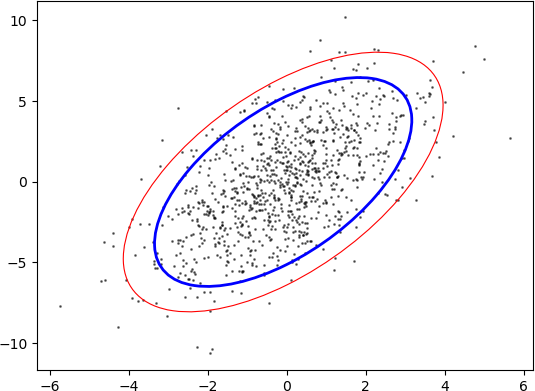
\includegraphics[height=2.5cm]{img/covariance.png}}

\begin{document} 

\maketitle

\begin{frame}{Table of contents}
  \setbeamertemplate{section in toc}[sections numbered]
  \tableofcontents%[hideallsubsections]
\end{frame}

\section[Intro]{Introduction}

\begin{frame}[fragile]{Measurement Errors}
  Can we improve vision algorithms by modeling inexact measurements?

  \begin{itemize}
  \item Errors accumulate during measurement. 
  \item Vision algorithms assume measurements are exact.
  \item Photogrammetry typically incorporates error analysis.
  \end{itemize}
\end{frame}

\begin{frame}[fragile]{Random Errors}
  \begin{definition}{Random errors} in experimental measurements are caused by unknown and unpredictable changes in the experiment.
  \end{definition}

  \begin{itemize}
    \item Errors are introduced by the feature extractor or the environmental conditions.
    \item An example of a source of random error is CCD noise.
  \end{itemize}
\end{frame}

\begin{frame}[fragile]{Modeling Random Errors}
  We assume that our feature extractors do not have systematic error,
  or that they are unbiased estimators.
  
  \begin{itemize}
  \item Measurements are modeled as random variables.
  \item The measurement is the sum of many unobserved random factors.
  \item The Central Limit Theorem is used to justify the
    representation of measurements as Gaussian random vectors.
  \end{itemize}
\end{frame}

\section{Covariance Propagation}

\begin{frame}[fragile]{Linearly Transforming a Distribution}
  \begin{theorem}
    Suppose $\vbX \sim p_{\vbX}(\vbx)$ and $\vbJ$ is an an invertible matrix. Then the 
    density of $\vbY = \vbJ\vbX$ is 
    \[p_{\vbY}(\vby) = \frac{p_{\vbX} \left(\vbJ^{\inv} \vby\right)}{|\det \vbJ|} \]
  \end{theorem}
\end{frame}

\begin{frame}[fragile]{Linear Transformation of a Gaussian is Gaussian}
  \begin{theorem}
    Suppose $\vbX \sim \mathcal{N}(\vbmu_{\vbX},\Sigma_{\vbX})$ and
    $\vbJ$ is an an invertible matrix. Then the density of $\vbY =
    \vbJ\vbX$ is
    \begin{align*}
      p_{\vbY}(\vby) &= \frac{p_{\vbX}(\vbJ^{\inv}\vby)}{| \det \vbJ |}  \\
      &= \mathcal{N}(\vbJ\vbX,\vbJ\Sigma_{\vbX}\vbJ^{\T})  \\
      &= \mathcal{N}(\vbY,\Sigma_{\vbY})  \\
    \end{align*}
  \end{theorem}
\end{frame}

\begin{frame}[fragile]{Explicit Covariance Propogation}
  Suppose $\vby = \vby(\vbx)$ and let $\vbx = \mu_{\vbx}+\Delta\vbx$. Linearize $\vby$ about $\mu_{\vbx}$,
  \[
  \vby(\mu_{\vbx}+\Delta\vbx)=\vby(\mu_{\vbx})+\vbJ_{\vby}(\mu_{\vbx})\Delta \vbx + \mathcal{O}(\|\Delta\vbx\|^2)
  \]

  Start with the definition of the covariance for the output $\vby$
  \begin{align*}
    \Sigma_{\vby} &= \mathbb{E}\left[(\vby-\mu_{\vby})(\vby-\mu_{\vby})^{T}\right] \\
    &= \mathbb{E}\left[\left(\vby(\mu_{\vbx}+\Delta\vbx)-\mu_{\vby}\right)\left(\vby(\mu_{\vbx}+\Delta\vbx)-\mu_{\vby}\right)^{T}\right] 
  \end{align*}

  Assume $\mu_{\vby} \approx \vby(\mu_{\vbx})$ and $\vby(\mu_{\vbx}+\Delta\vbx) \approx \vby(\mu_{\vbx})+\nabla \vby(\mu_{\vbx})\Delta \vbx$, then 
  \begin{align*}
    \Sigma_{\vby} & \approx \mathbb{E}\left[\left(\vby(\mu_{\vbx}+\Delta\vbx)-\vby(\mu_{\vbx})\right)\left(\vby(\mu_{\vbx}+\Delta\vbx)-\vby(\mu_{\vbx})\right)^{T}\right] \\
    & \approx \mathbb{E}\left[\vbJ_{\vby}(\mu_{\vbx})\Delta\vbx\Delta\vbx^{\T}\vbJ_{\vby}(\mu_{\vbx})^{\T}\right] \\
    & \approx \vbJ_{\vby}(\mu_{\vbx})\Sigma_{\vbx}\vbJ_{\vby}(\mu_{\vbx})^{\T}
  \end{align*}
  
  $\mu_{\vbx}$ is unknown, but if $\Delta\vbx$ is small
  \begin{equation}
    \label{eq:cov_prop}
    \Sigma_{\vby} \approx \vbJ_{\vby}(\vbx)\Sigma_{\vbx}\vbJ_{\vby}(\vbx)^{\T}.
  \end{equation}
\end{frame}

\begin{frame}[fragile]{Implicit Function Theorem}
  \begin{theorem}[Implicit function]
    \label{thm:implicit_function}
    Let $\vbphi(\vbx,\vbz): \Re^m \times \Re^n \to \Re^n$ be an
    implicit function and suppose that
    \begin{enumerate}[(i)]
    \item $(\vbx,\vbz) \in \Re^m\times\Re^n$,
    \item function $\vbphi$ is differentiable,
    \item $\vbphi(\vbx_i,\vbz^*)=\vbzero$, and
    \item $\det \pdv{\vbphi}{\vbz}_{(\vbx,\vbz^*)} \neq 0$.
    \end{enumerate}
    Then there is the unique and differentiable function $\vbz(\vbx)$ in the open neighborhood of
    $(\vbx,\vbz^*)$ so that $\vbphi(\vbx, \vbz(\vbx))=\vbzero$.
  \end{theorem}

  \smallskip
  
  \begin{remark}
    Suppose that $\vbphi$ satisfied the sufficient conditions to
    invoke the Implicit Function Theorem. Then we compute an expression
    for $\odv{\vbz}/{\vbx}$ without knowing the functional form of
    $\vbz(\vbx)$. 
  \end{remark}
\end{frame}

\begin{frame}{Implicit Differentiation}
  \begin{theorem}
    \label{corr:implicit_diff}
    Let $\vbz(\vbx): \Re^m \to \Re^n$ and implicitly defined by
    $\phi(\vbx,\vbz)=\vbz-\vbz(x)=\vbzero$ and suppose that $\vbphi$ satisfies the sufficient
    conditions of \eqref{thm:implicit_function}. Then $\odv{\vbz}{\vbx}$
    exists and is computable.
  \end{theorem}

  \begin{proof}
  Impilcitly differentiate $\vbphi$
  \[
    \odv{\vbphi}{\vbx} = \pdv{\vbphi}{\vbx}+\pdv{\vbphi}{\vbz}\odv{\vbz}{\vbx} = \vbzero,
  \]
  and solve for $\odv{\vbz}/{\vbx}$
  \[
    \odv{\vbz}{\vbx} = -\pdv{\vbphi}{\vbz}^{\inv}\pdv{\vbphi}{\vbx}
  \]
  to compute its functional form.
\end{proof}
\end{frame}

\begin{frame}{Regression}
  \begin{problem}[Optimization]
    Given $\vbx$ and a differentiable function $\mathcal{J}$, solve for
    parameters $\vbz^{*}$ such that
    \[
      \label{eq:minimization_problem}
      \vbz^{*} = \argmin_{\vbz} \mathcal{J}(\vbx,\vbz).
    \]
  \end{problem}

  \smallskip

  \begin{definition}[First-order optimality]
    The constraint
    \[
      \pdv{\mathcal{J}}{\vbz}_{(\vbx,\vbz^*)} = \vbzero^{\T}.
    \]
    must be satisfied for $\vbz^*$ to be locally optimal.
  \end{definition}

  \smallskip

  \begin{desiderata}[Parameter uncertainty]
    Referring to \eqref{eq:cov_prop}, we need to compute
    $\odv{\vbz}/{\vbx}$ to propagate errors from measurements to
    parameters.
  \end{desiderata}
\end{frame}


\begin{frame}[fragile]{Uncosntrained Minimization}
  Suppose $\vbz^*$ is a local minimizer of the objective
  $\mathcal{J}(\vbx,\vbz)$. Then we have the first-order optimality
  condition
  \[
    \pdv{\mathcal{J}}{\vbz}_{(\vbx,\vbz^*)}=\vbzero^{\T}.
  \]

  \smallskip
  
  Applying \eqref{corr:implicit_diff}, we have
  \begin{equation}
    \odv{\vbz}{\vbx} = \left(\pdv[order=2]{\mathcal{J}}{\vbz}\right)^\inv\pdv{\mathcal{J}}{\vbz,\vbx}
  \end{equation}

  \smallskip
  
  For concision, we use the matrix notations for Jacobain and Hessian going forward,
  \begin{equation}
    \label{eq:dz_dx}
    \vbJ_{\vbz} = \odv{\vbz}{\vbx} \qquad \vbH_{\mathcal{J}} =\pdv[order=2]{\mathcal{J}}{\vbz}.
  \end{equation}
\end{frame}

\begin{frame}{Covariance Propagation}
  \begin{remark}
    We obtain the functional form of $\vbJ_{\vbz}$ from
    \eqref{eq:dz_dx} even though we don't know $\vbz(\vbx)$.
  \end{remark}
  
  We can substitute $\vbJ_z$ into \eqref{eq:cov_prop} to compute the
  uncertainty of the parameters,
  \[
    \vbSigma_{\vbz} = \vbJ_z \vbSigma_{\vbx}\vbJ^{\T}_z.
  \]
\end{frame}

\begin{frame}{Scale Equivariance of Covariance}
  \begin{lemma}
    Suppose that minimizer $\vbz$ has covariance $\vbSigma_{\vbz}$.
    Then $\alpha \vbz$ has covariance $\alpha^2 \vbSigma_{\alpha}$.
  \end{lemma}
  \begin{proof}
  \[
    \begin{split}
      \vbSigma_{\alpha\vba} &= \EE\brackets{(\alpha\vba-\alpha\bar{\vba})(\alpha\vba-\alpha\bar{\vba})} \\
                            &= \EE\brackets{ \alpha^2(\vba-\bar{\vba})(\vba-\bar{\vba})} \\
                            &= \alpha^2 \EE\brackets{ (\vba-\bar{\vba})(\vba-\bar{\vba}) } \\
                            &= \alpha^2\EE\brackets{\vbSigma_{\vba}}
    \end{split}
  \]
\end{proof}

\begin{remark}
  How does this arbitrary scale propagate? How does it affect downstream hypothesis tests?
\end{remark}
\end{frame}

\begin{frame}{Rank-deficient Covariance Matrices}
  Covariance in the direction of a homogeneous vector is 0 since 
  it is arbitrary. This is captured by enforcing
  \[
    \vbSigma_{\vbz}\vbz = \vbzero.
  \]
\end{frame}
  
%\begin{frame}[fragile]{Gauss-Newton Approximation to the Hessian}
%  Suppose $\mathcal{J}(\vbx,\vby)=\|\ve(\vbx,\vby)\|_2^2$.
%  \vspace{1em}y
%  Then
%  \[
%  \vbH_{\mathcal{J}} = 2\left(\vbJ^{\T}_{\mathcal{J}}\vbJ_{\mathcal{J}}+\sum_i e_i(\vbx,\vby)^{\T} \right)
%  \]
%\end{frame}
%
%\begin{frame}
%  Then (1) can be applied to propogate the covariance
%
%  \begin{equation}
%    \Sigma_{\vby} \approx \vbJ_{\vby}(\vbx)\Sigma_{\vbx}\vbJ_{\vby}(\vbx)^{\T}.
%  \end{equation}
%\end{frame}

\begin{frame}
  \begin{remark}
    The fundamental matrix $\vbF$ is a rank-two matrix that relates
    point correspondences $\set{\cspond{\vbx_i}{\vbx'_i}}$ in
    stereo images.
  \end{remark}
  
  \smallskip
  
  For noiseless measurements, the epipolar line
  \[
    \vbl' = \vbF\vbx
  \]
  in the second image contains $\vbx'$
  \[
    \vbl'^{\T}\vbx' = 0.
  \]
\end{frame}

\begin{frame}[fragile]{Seven-point Method}
  This epipolar constraint $\vbx^{'\T} \vbF \vbx=0$ can be written as
  \[
    \label{eq:F_constraint}
    \vbm^\T_i \vect \vbF = \vbx_i \otimes \vbx'_i  \vect \vbF = 0.
  \]

  \smallskip
  
  \begin{enumerate}[(i)]
  \item Homogeneous constraints of the form \eqref{eq:F_constraint} are
    stacked in a design matrix.
  \item $\vbF$ has 7 degrees of freedom, so 7 equations are needed.
  \end{enumerate}

  \smallskip
  
  Letting $\vbz = \operatorname{vec}(\vbF^{\T})$ we have
  \[
    \label{eq:sevenpt_linear}
    \vbM\vbz = \vbzero,
  \]
  where $\vbM \in \mathcal{M}_{7 \times 9}(\Re)$.

  \begin{result}
    The two-dimensional kernel of $\vbM$ contains either one or three
    solutions for the fundamental matrix.
  \end{result}
\end{frame}
 
\begin{frame}[fragile]{Imposing Rank Two Constraint}
  Denote the basis vectors of $\ker(\vbM)$ as $\vbf_1$ and $\vbf_2$.

  \smallskip
  
  $\vbF$ is singular, so
  \begin{equation}
    \label{eq:Fcubic_eq}
    \det \operatorname{vec}^{\inv}_{3\times3} (\vbf_1+\alpha_i \vbf_2) = 0.
  \end{equation}

  \smallskip
  
  There are either one or three roots to the cubic induced by
  \eqref{eq:Fcubic_eq}, which are used to construct the solutions
  \begin{equation}
    \label{eq:estimateF}
    \vbF_i = \operatorname{vec}^{\inv}_{3\times3} (\vbf_1+\alpha_i \vbf_2)^{\T}.
  \end{equation}

  Let $\vbF \in \{ \vbF_i \}$ be a solution.
  \medskip

  Matrix $\lambda \vbF^{*}_i$ is also a solution to \eqref{eq:sevenpt_linear} for nonzero $\lambda$.
\end{frame}

\begin{frame}{Covariance Propagation}
  \medskip
  
  Restrict solutions to lie on the hypersphere
  \[
    \vbF^{*} = \frac{\vbF}{\| \vbF^{*} \|}
  \]
  Consider the constraint equations as residuals, namely
  \[
  \mathcal{J}(\vbx,\vbf)= \| \vbM\vbf \|^2 = \|\vbepsilon \|^2 = \sum_i \vbepsilon_i^2  = \sum_i \| \vbx[i]^{\prime \T} \vbF \vbx[i] \|^2
  \]
  
  Let $\vbF^{*}$ be computed for measurements $\vbx_0$ by the seven-point method.
  \bigskip

  $\mathcal{J}(\vbx_0,\vbf^*)$ is 0, so  $\pdv*{\mathcal{J}(\vbx,\vbf)}{\vbf}{(\vbx_0,\vbf^*)} = \vbzero$.
\end{frame}

%\begin{frame}
%  $\vbf^*$ is not a minimal parameterization.
%  \bigskip
%
%  We must account for the rank-two constraint and scale ambiguity.
%  \bigskip
%  
%  Let $\alpha,\beta \in \Re$ amd $g_2 \in \Re^3$ and $g_3 \in \Re^2$, and $g_1 = \alpha g_2 + \beta \cvec{g_3,f_{33}}$
%
%  Then parameter vector $\theta = \rvec{\alpha,\beta,g_2,g_3}$
%  \[
%    \vbf(\theta) = \cvec{g_1,g_2,g_3,f_{33}}
%  \]
%  
%  and the objective becomes $\mathcal{J}(\vbx,\theta)$
%\end{frame}
%
%\begin{frame}
%  \begin{equation}
%    \vbJ_{\theta} = \pdv{\mathcal{J}}{\theta}^{\inv}\pdv{\mathcal{J}}{\theta \vbx}
%  \end{equation}
%  \bigskip
%  where $\vbJ_{\theta} \in \Re^{7 \times 28}$ so that $\vbSigma_\theta = \vbJ_{\theta}\vbSigma_{\vbx}\vbJ^\T_{\theta} $
%
%  \bigskip
%  and
%
%  \bigskip
%  $\vbJ_{\vbf} = \odv{\vbf}{\theta}$ so that  $\Sigma_f = \vbJ_{\vbf} \Sigma_{\theta} \vbJ^{\T}_{\vbf}$.
%
%
%\end{frame}

\end{document}
